\documentclass[a4paper,14pt]{article} % тип документа
%\documentclass[14pt]{extreport}
\usepackage{extsizes} % Возможность сделать 14-й шрифт


\usepackage{geometry} % Простой способ задавать поля
\geometry{top=20mm}
\geometry{bottom=25mm}
\geometry{left=15mm}
\geometry{right=15mm}

\setcounter{section}{0}

%%%Библиотеки
%\usepackage[warn]{mathtext}
%\usepackage[T2A]{fontenc} % кодировка
\usepackage[utf8]{inputenc} % кодировка исходного текста
\usepackage[english,russian]{babel} % локализация и переносы
\usepackage{caption}
\usepackage{listings}
\usepackage{amsmath,amsfonts,amssymb,amsthm,mathtools}
\usepackage{wasysym}
\usepackage{graphicx}%Вставка картинок правильная
\usepackage{float}%"Плавающие" картинки
\usepackage{wrapfig}%Обтекание фигур (таблиц, картинок и прочего)
\usepackage{fancyhdr} %загрузим пакет
\usepackage{lscape}
\usepackage{xcolor}
\usepackage{dsfont}
%\usepackage{indentfirst}
\usepackage[normalem]{ulem}
\usepackage{hyperref}




%%% DRAGON STUFF
\usepackage{scalerel}
\usepackage{mathtools}

\DeclareMathOperator*{\myint}{\ThisStyle{\rotatebox{25}{$\SavedStyle\!\int\!\!\!$}}}

\DeclareMathOperator*{\myoint}{\ThisStyle{\rotatebox{25}{$\SavedStyle\!\oint\!\!\!$}}}

\usepackage{scalerel}
\usepackage{graphicx}
%%% END 

%%%Конец библиотек

\newcommand{\drawsome}[1]{            % Для быстрой вставки картинок
    \begin{figure}[h!]
            \centering
            \includegraphics[scale=0.7]{#1}
            \label{fig:first}
    \end{figure}
}
\newcommand{\drawsomemedium}[1]{
    \begin{figure}[h!]
            \centering
            \includegraphics[scale=0.45]{#1}
            \label{fig:first}
    \end{figure}
}
\newcommand{\drawsomesmall}[1]{
    \begin{figure}[h!]
            \centering
            \includegraphics[scale=0.3]{#1}
            \label{fig:first}
    \end{figure}
}

%%%Настройка ссылок
\hypersetup
{
colorlinks=true,
linkcolor=blue,
filecolor=magenta,
urlcolor=blue
}
%%%Конец настройки ссылок


%%%Настройка колонтитулы
	\pagestyle{fancy}
	\fancyhead{}
	\fancyhead[L]{Домашнее задание}
	\fancyhead[R]{Крейнин Матвей, группа Б05--005}
	\fancyfoot{}
    \fancyfoot[C]{\thepage}
    \fancyfoot[R]{ТРЯП}
%%%конец настройки колонтитулы


\begin{document}
%%%%Начало документа%%%%

\section{Задание 7}
\subsection{Задача 1}
Построим суффиксный автомат $\mathcal{A}$ по алгоритму, вот разные его стадии.

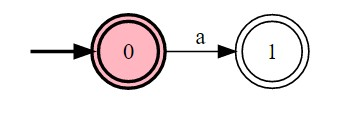
\includegraphics{01.jpg}

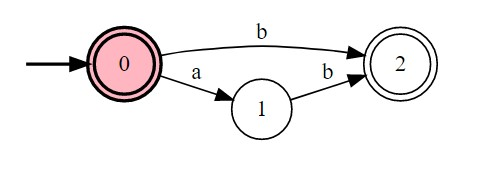
\includegraphics{02.jpg}

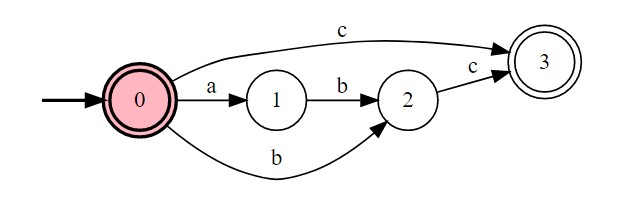
\includegraphics{03.jpg}

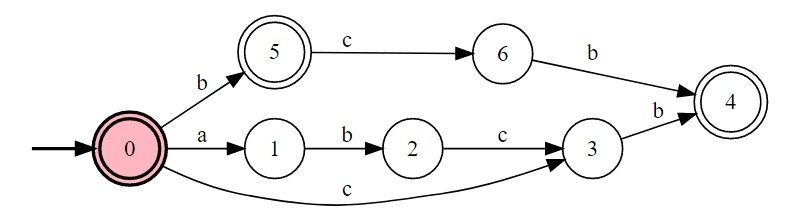
\includegraphics{04.jpg}

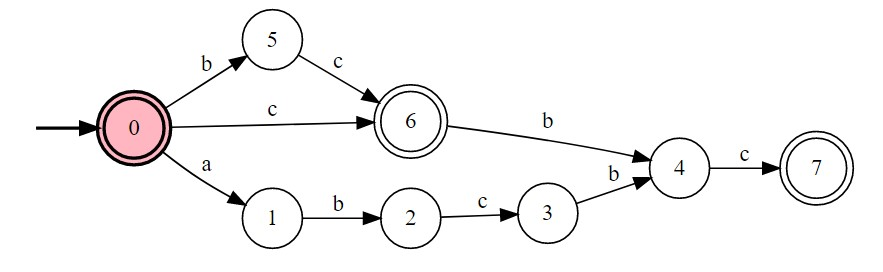
\includegraphics{05.jpg}

\textbf{1.} Минимальное количество раз, если только будет встречаться в подсловах bcbc по одному разу и ни в каких других больше, получится 20 раз.
Максимальное количество раз, если припишем к каждому bcbc по c в начале, получим 40 раз, и припишем к оставшемся 20 bc c в начало, получим еще 20 раз. Итого максимум получится 60 раз.

\underline{Ответ:} от 20 до 60 раз включительно.
\newline
\textbf{2.} Т.к. $\epsilon \in Suff(abcbc)$, то получается, что это вообще любое слово, но будем считать, что это не так.
\newline
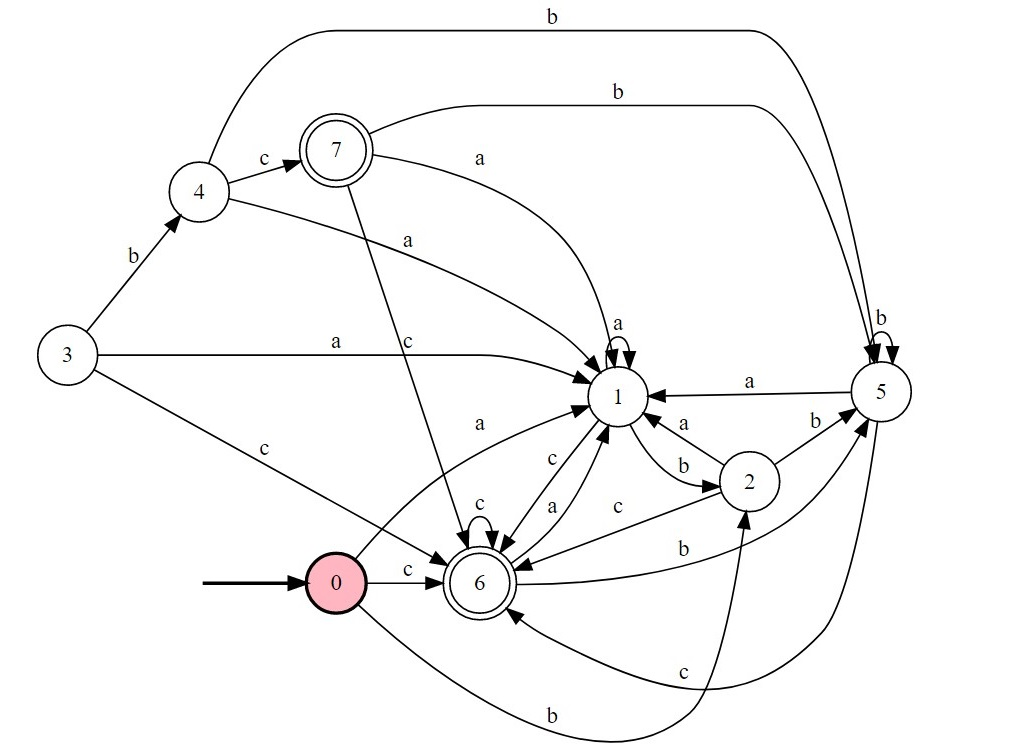
\includegraphics[scale=0.95]{06.jpg}

Но вообще, это всё что угодно, что заканчивается на c, поэтому ДКА выглядит вот так:

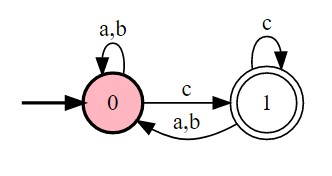
\includegraphics{07.jpg}

\textbf{3.} Coming soon...

\subsection{Задача 2}
\textbf{1.} X = ((110)* +111*)X.
\newline
\textbf{а) 111} \textbf{б) $((110)^*|111^*)^*$} \textbf{в) $((110)^*|111^*)^*$}
\newline
\textbf{2.} X = (00 + 01 + 10 + 11)X + (0 + 1 + $\varepsilon$)
\newline
\textbf{а) 0} 
\textbf{б) $(00|01|10|11)^*(0|1|\varepsilon)$} 
\textbf{в) $(\Sigma \Sigma)^*(0|1|\varepsilon)$ $=$ $\Sigma^*$}
\newline
\textbf{3.} 
\begin{equation*}
     \begin{cases}
       \text{$Q_0$ = 0$Q_0$ + 1$Q_1$ + $\varepsilon$}\\
       \text{$Q_1$ = 1$Q_0$ + 0$Q_2$}               \\
       \text{$Q_2$ = 0$Q_0$ + 1$Q_2$}
     \end{cases}
\end{equation*}

\textbf{а) частное решение}
\textbf{б) решение, минимальное по включению}
\textbf{в) все решения}

\end{document}